\documentclass[conference,a4paper]{IEEEtran}
% conference: differentiate between journals and conference format
% a4paper: set the paper size to A4
%% Support sites:
%% http://www.michaelshell.org/tex/ieeetran/
%% http://www.ctan.org/tex-archive/macros/latex/contrib/IEEEtran/
%% and
%% http://www.ieee.org/

%\IEEEoverridecommandlockouts
% The preceding line is only needed to identify funding in the first footnote. If that is unneeded, please comment it out.

%% Package inclusion
%% More details on what many of these packages do are at the end of this file
\usepackage[T1]{fontenc}%T1 fonts have Þ and ð
\usepackage[utf8]{inputenc}% allows UTF encoding, needed for Icelandic characters


\usepackage{cite}%reorganizing citation numbers
\usepackage[cmex10]{amsmath}%American Math Society(AMS) math formatting
\usepackage{amssymb,amsfonts}%AMS extra symbols and fonts
\interdisplaylinepenalty=2500%allow line breaks in multi-line formulas
\usepackage{array}%enhanced table tools
\usepackage[caption=false,font=footnotesize]{subfig}%sub-figures under a main figure
\usepackage{dblfloatfix}%fix double column figure ordering and placement

\usepackage{algorithmic}%writing algorithms
\usepackage{graphicx}%graphics inclusion
% declare the path(s) where your graphic files are
\graphicspath{{graphics/}{moregraphics/}}
% and their extensions so you won't have to specify these with
% every instance of \includegraphics
\DeclareGraphicsExtensions{.pdf,.PDF,.jpeg,.JPEG,.jpg,.JPEG,.png,.PNG}

\usepackage{booktabs}%pretty lines in tables: \toprule,\columnrule,\bottomrule

\usepackage{siunitx}%SI unit formatting:  \SI{9.8}{\meter\per\second} and \si{\meter\per\second\square}

\usepackage{textcomp}%special symbols not in all fonts
\usepackage{xcolor}%color macros
\usepackage[spaces,hyphens]{url}
\usepackage{float}


% *** Do not adjust lengths that control margins, column widths, etc. ***
% *** Do not use packages that alter fonts (such as pslatex).         ***
% There should be no need to do such things with IEEEtran.cls V1.6 an   d later.
% (Unless specifically asked to do so by the journal or conference you plan
% to submit to, of course. )

\begin{document}

\title{Understanding of Modern Software-Defined Networking}

\author{\IEEEauthorblockN{Phong Ngoc Hoang Nguyen}
\IEEEauthorblockA{nhphong.nguyen@mail.utoronto.ca \\ University of Toronto}
}

\maketitle
\begin{abstract}
    This report summarizes an investigation of modern Software-Defined Networking (SDN), focusing on the evolution from the traditional network architecture, where the control plane and data plane are tightly coupled within individual network devices, to early SDN architecture that separate network control from packet forwarding, and ultimately to modern programmable network infrastructures deployed in large-scale data centers. The study examined ONOS, P4, Stratum, P4Runtime and Leaf-Spine Fabric. Particular attention was given to the separation of control and data planes, controller abstractions, programmable forwarding pipelines, and production-scale fabric architectures. The report concludes with some of the use cases, observations on the architectural tradeoffs and research challenges associated with programmable networks.
\end{abstract}

\begin{IEEEkeywords}
Computer Network, Software-Defined Network, SDN
\end{IEEEkeywords}

\section{Introduction}
Started back in 1952, when IBM first manufactured large computer system and sold into the market as mainframe. It was bulky, large, and expensive machine that take up a room size. More importantly, every components within that mainframe is IBM's proprietary hardware, which means, a customer have to buy the whole vertically integrated solution from a single vendor regardless of the solution they want to have for their problem (software calculation, hardware design, finance...).
\begin{figure}[H]
    \centering
    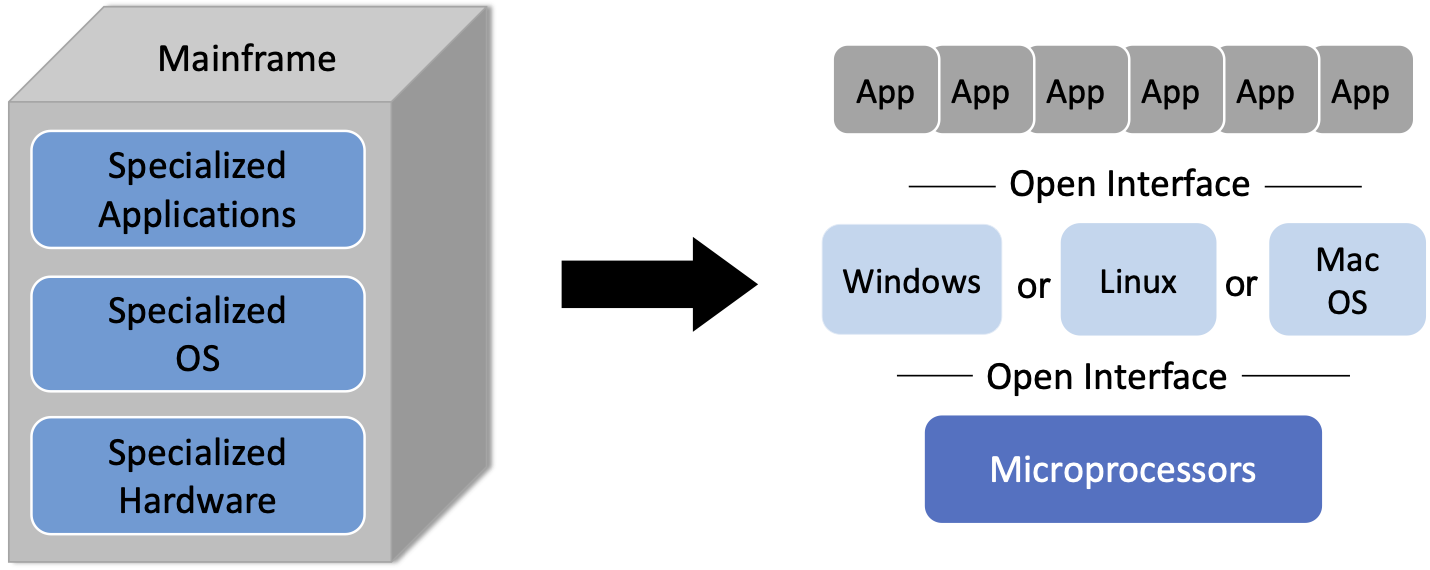
\includegraphics[width=1\linewidth]{graphics/vertical integrated solution.png}
    \caption{Transformation from vertical market to horizontal marketplace with open interfaces at all level}
    \label{fig:placeholder}
\end{figure}
The evolution began with the arrival of open-source operating systems and microprocessors, which helped transform the market into a horizontal one where innovation could happen at any layer.

SDN initiatives draw the similar inspiration by decoupling the control plane from the data plane. Decision-making logic is decided by a external\footnote{In SDN terminology, a distinction exists between \textbf{external (global) network OS} and the \textbf{internal (local) network OS}. The External NOS referrs to a distributed controller platform to maintain a centralized view of the network (ONOS section) while Internal OS refers to lightweight OS running directly on-switch to manage internal switch operation and communicate with the external network OS.} logically centralized controller\footnote{While SDN control plane is logically centralized to provide a unified global view of network state and simplify network management, production deployment (introduced in ONOS section) are physically distributed for high availability and scalability}, using information from network operating systems enabled on top of the underlying switches. This abstraction simplifies switch's role, off-loading complex decision making logic (i.e., routing, path computation, ACL..) off-device and reducing the switch's primary task to packet forwarding. So they are referred to as "white box" or "bare-metal" switches\footnote{"bare-metal" switches run a ONIE bootloader uses facilities in Linux kernel and BusyBox, defining an open source "install environment" for end users to install target network OS} which doesn't come with a fixed network OS, creating a hardware ecosystem for multiple operating system vendors.

OpenFlow is the pioneer protocol that support this disaggregation in the early stage of SDN. Although it was a main instrumental propelling SDN into the mainstream, OpenFlow now play a small role of today SDN because of an architectural limitation it imposed---namely, its fixed-function match-action pipeline. Modern infrastructure has largely transitioned toward fully programmable data planes driven by the P4 programming language, P4Runtime, and Stratum. The objective of this study is to explore this architectural evolution from early OpenFlow to current P4-based ecosystems deployed across large-scale hyperscale data centers.

\section{Basic Architecture}
The core philosophy of Software-Defined Networking is horizontal disaggregation across every layers of the networking stack. Rather than relying on a vertically integrated, propriety hardware appliances, SDN decompose them into abstract components that is independent from other components, allowing each of which being used interchangeably and innovated at each layer.
\begin{itemize}
    \item \textbf{Local Network OS layer:} Physical switch hardware is decoupled from proprietary vendor software through bare-metal whitebox switches. Utilizing an Open Network Install Environment (ONIE) bootloader, the switch can load any compatible local Network OS (e.g., Stratum, SONiC) to handle local hardware initialization and peripheral management.
    \item \textbf{Control-to-Data Communication Interface:} The control plane and data plane interact over well-defined consumer/provider API endpoints using standard protocol (e.g. OpenFlow, gRPC/P4Runtime). This bidirectional interface allows controller to program forwarding rules while collecting real-time telemetry, link states, metrics, and packet from the data plane.
    \item \textbf{Device Driver \& Pipeline Layer:} This layer resolves hardware heterogeneity by splitting device control into low-level driver abstractions and pipeline-mapping logic. Analogous to a hardware SDK, the \textit{device driver} handles low-level chip management, translate control protocol messages (e.g., OpenFlow or P4Runtime) directly into chip memory while absorbing vendor-specific behavior mismatches. Sitting above the driver, the \textit{pipeliner} maps generic, high-level \textit{flow objectives} into the exact multi-table forwarding pipeline required by the underlying ASIC, freeing higher-layer application logic from needing to know the switch's internal table layout.
    \item \textbf{Data Plane layer: } Packet processing logic is completely decoupled from fixed-function hardware ASIC pipeline, allowing enterprise to implement custom header protocols on demand instead of waiting for switch vendor for the protocol implementation in their silicon chips. Using P4 language, packet parsing, header modifications, and forwarding behaviors can be programmed, updated, and recompiled directly on the hardware at runtime.
\end{itemize}
\subsection{Single-switch perspective: The Software Stack}
This includes an overview of a SDN stack with the involvement of a switch and controllers, highlight the top-to-bottom software stack being used in the SDN architecture. The main component include the Control App, Network OS, Switch OS, and P4 program--which used for the programmable switch. Figure 2 also introduced an exemplar of open-source software we used for this report (e.g. SD-Fabric, ONOS, Stratum), and protocol uses for communication between each layer. 
\begin{figure}[H]
    \centering
    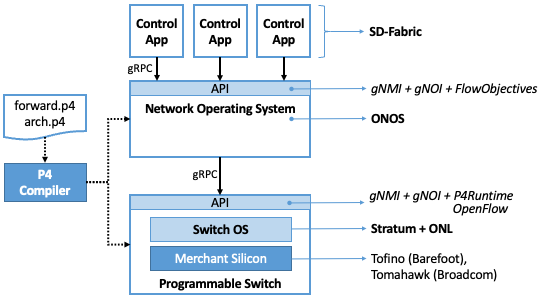
\includegraphics[width=1\linewidth]{graphics/image.png}
    \caption{Overall architecture of SDN stack with one switch}
    \label{fig:placeholder}
\end{figure}
At the top of the stack, Control Applications communicate with the Network OS via gRPC over Northbound APIs. Rather than writing raw table entries, applications issue high-level, topology-agnostic \textit{Intent}, or hardware-agnostic routing intents called \textit{Flow Objectives} (e.g., policy constraints or forwarding goals). Concurrently, management interfaces such as gNMI (gRPC Network Management Interface) and gNOI (gRPC Network Operations Interface) are exposed on the Northbound interface, enabling control applications to query dynamic network state (e.g., topology graphs, link statuses) and execute operational lifecycle commands (e.g., rebooting or upgrading devices).

Below the control abstraction is the separation of the control plane and the data plane. The Network OS compiles high-level Flow Objectives into low-level, device-specific \textit{Flow Rules}—concrete match-action entries targeted at explicit hardware table from the entire hardware pipeline. These rules are pushed down via gRPC using southbound protocols such as P4Runtime, OpenFlow, or gNMI. Upon receiving these instructions, the local Switch OS (e.g., Stratum, originally developed by Google) programs the entries directly into the hardware switch silicon\footnote{Switch silicon refers to a specialized integrated circuit (ASIC) designed for line-rate packet processing, switching, and hardware-accelerated QoS management.}. Popular commercial implementations of this merchant silicon include Intel's Barefoot Tofino and Broadcom's Tomahawk chips.
\subsection{Network-Wide perspective: The Entire Network Data Path}
\begin{figure}[H]
    \centering
    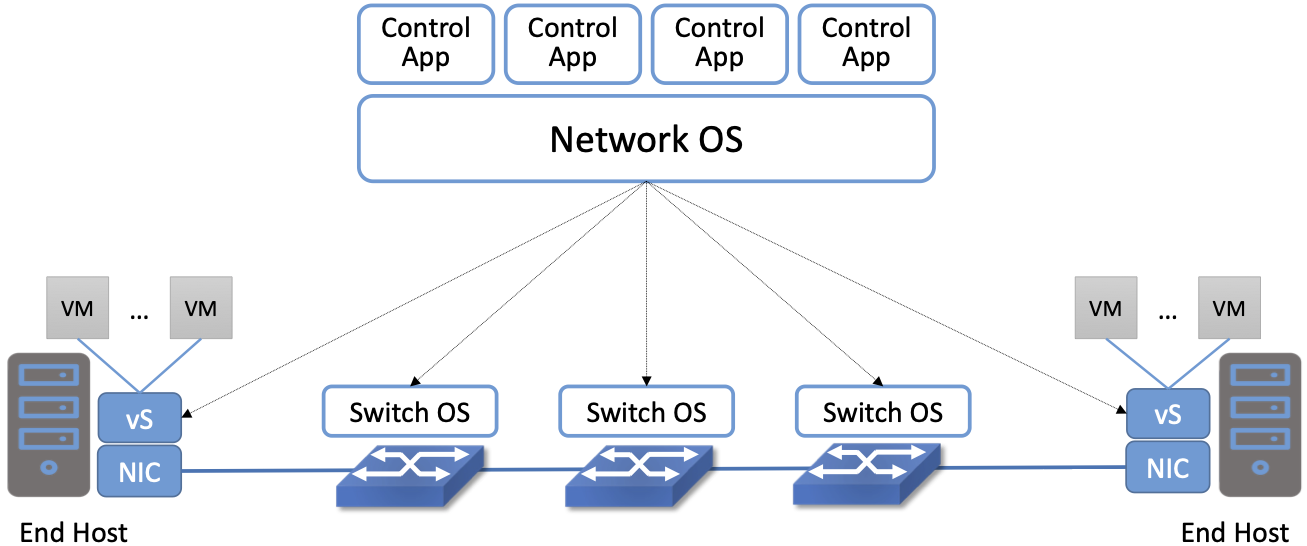
\includegraphics[width=1\linewidth]{graphics/network-wide sdn.png}
    \caption{End-End network view of SDN architecture}
    \label{fig:placeholder}
\end{figure}
\section{Bare-metal switches and P4 programmable data plane}
\section{Switch OS}
\section{Network OS}\label{sec:onos}
\section{Leaf-spine Fabric}
\section{Research Direction}

\end{document}
%%% Description for the packages used at the beginning of this file


%\usepackage{cite}
% cite.sty was written by Donald Arseneau
% V1.6 and later of IEEEtran pre-defines the format of the cite.sty package
% \cite{} output to follow that of IEEE. Loading the cite package will
% result in citation numbers being automatically sorted and properly
% "compressed/ranged". e.g., [1], [9], [2], [7], [5], [6] without using
% cite.sty will become [1], [2], [5]--[7], [9] using cite.sty. cite.sty's
% \cite will automatically add leading space, if needed. Use cite.sty's
% noadjust option (cite.sty V3.8 and later) if you want to turn this off
% such as if a citation ever needs to be enclosed in parenthesis.
% cite.sty is already installed on most LaTeX systems. Be sure and use
% version 4.0 (2003-05-27) and later if using hyperref.sty. cite.sty does
% not currently provide for hyperlinked citations.
% The latest version can be obtained at:
% http://www.ctan.org/tex-archive/macros/latex/contrib/cite/
% The documentation is contained in the cite.sty file itself.





%% Setup graphics inclusion
%\usepackage{graphicx}
% declare the path(s) where your graphic files are
%\graphicspath{{../pdf/}{../jpeg/}}
% and their extensions so you won't have to specify these with
% every instance of \includegraphics
%\DeclareGraphicsExtensions{.pdf,.PDF,.jpeg,.JPEG,.jpg,.JPEG,.png,.PNG}

% graphicx was written by David Carlisle and Sebastian Rahtz. It is
% required if you want graphics, photos, etc. graphicx.sty is already
% installed on most LaTeX systems. The latest version and documentation
% can be obtained at: 
% http://www.ctan.org/tex-archive/macros/latex/required/graphics/
% Another good source of documentation is "Using Imported Graphics in
% LaTeX2e" by Keith Reckdahl which can be found at:
% http://www.ctan.org/tex-archive/info/epslatex/
%
% latex, and pdflatex in dvi mode, support graphics in encapsulated
% postscript (.eps) format. pdflatex in pdf mode supports graphics
% in .pdf, .jpeg, .png and .mps (metapost) formats. Users should ensure
% that all non-photo figures use a vector format (.eps, .pdf, .mps) and
% not a bitmapped formats (.jpeg, .png). IEEE frowns on bitmapped formats
% which can result in "jaggedy"/blurry rendering of lines and letters as
% well as large increases in file sizes.
%
% You can find documentation about the pdfTeX application at:
% http://www.tug.org/applications/pdftex

% *** MATH PACKAGES ***
%
%\usepackage[cmex10]{amsmath}
% A popular package from the American Mathematical Society that provides
% many useful and powerful commands for dealing with mathematics. If using
% it, be sure to load this package with the cmex10 option to ensure that
% only type 1 fonts will utilized at all point sizes. Without this option,
% it is possible that some math symbols, particularly those within
% footnotes, will be rendered in bitmap form which will result in a
% document that can not be IEEE Xplore compliant!
%
% Also, note that the amsmath package sets \interdisplaylinepenalty to 10000
% thus preventing page breaks from occurring within multiline equations. Use:
%\interdisplaylinepenalty=2500
% after loading amsmath to restore such page breaks as IEEEtran.cls normally
% does. amsmath.sty is already installed on most LaTeX systems. The latest
% version and documentation can be obtained at:
% http://www.ctan.org/tex-archive/macros/latex/required/amslatex/math/


% *** ALIGNMENT PACKAGES ***
%
%\usepackage{array}
% Frank Mittelbach's and David Carlisle's array.sty patches and improves
% the standard LaTeX2e array and tabular environments to provide better
% appearance and additional user controls. As the default LaTeX2e table
% generation code is lacking to the point of almost being broken with
% respect to the quality of the end results, all users are strongly
% advised to use an enhanced (at the very least that provided by array.sty)
% set of table tools. array.sty is already installed on most systems. The
% latest version and documentation can be obtained at:
% http://www.ctan.org/tex-archive/macros/latex/required/tools/


% IEEEtran contains the IEEEeqnarray family of commands that can be used to
% generate multiline equations as well as matrices, tables, etc., of high
% quality.




% *** SUBFIGURE PACKAGES ***
%\usepackage[caption=false,font=footnotesize]{subfig}
% subfig.sty, written by Steven Douglas Cochran, is the modern replacement
% for subfigure.sty, the latter of which is no longer maintained and is
% incompatible with some LaTeX packages including fixltx2e. However,
% subfig.sty requires and automatically loads Axel Sommerfeldt's caption.sty
% which will override IEEEtran.cls' handling of captions and this will result
% in non-IEEE style figure/table captions. To prevent this problem, be sure
% and invoke subfig.sty's "caption=false" package option (available since
% subfig.sty version 1.3, 2005/06/28) as this is will preserve IEEEtran.cls
% handling of captions.
% Note that the Computer Society format requires a larger sans serif font
% than the serif footnote size font used in traditional IEEE formatting
% and thus the need to invoke different subfig.sty package options depending
% on whether compsoc mode has been enabled.
%
% The latest version and documentation of subfig.sty can be obtained at:
% http://www.ctan.org/tex-archive/macros/latex/contrib/subfig/




% *** FLOAT PACKAGES ***
%
%\usepackage{fixltx2e}
% fixltx2e, the successor to the earlier fix2col.sty, was written by
% Frank Mittelbach and David Carlisle. This package corrects a few problems
% in the LaTeX2e kernel, the most notable of which is that in current
% LaTeX2e releases, the ordering of single and double column floats is not
% guaranteed to be preserved. Thus, an unpatched LaTeX2e can allow a
% single column figure to be placed prior to an earlier double column
% figure. The latest version and documentation can be found at:
% http://www.ctan.org/tex-archive/macros/latex/base/


%\usepackage{stfloats}
% stfloats.sty was written by Sigitas Tolusis. This package gives LaTeX2e
% the ability to do double column floats at the bottom of the page as well
% as the top. (e.g., "\begin{figure*}[!b]" is not normally possible in
% LaTeX2e). It also provides a command:
%\fnbelowfloat
% to enable the placement of footnotes below bottom floats (the standard
% LaTeX2e kernel puts them above bottom floats). This is an invasive package
% which rewrites many portions of the LaTeX2e float routines. It may not work
% with other packages that modify the LaTeX2e float routines. The latest
% version and documentation can be obtained at:
% http://www.ctan.org/tex-archive/macros/latex/contrib/sttools/
% Do not use the stfloats baselinefloat ability as IEEE does not allow
% \baselineskip to stretch. Authors submitting work to the IEEE should note
% that IEEE rarely uses double column equations and that authors should try
% to avoid such use. Do not be tempted to use the cuted.sty or midfloat.sty
% packages (also by Sigitas Tolusis) as IEEE does not format its papers in
% such ways.
% Do not attempt to use stfloats with fixltx2e as they are incompatible.
% Instead, use Morten Hogholm'a dblfloatfix which combines the features
% of both fixltx2e and stfloats:
%
%\usepackage{dblfloatfix}
% The latest version can be found at:
% http://www.ctan.org/tex-archive/macros/latex/contrib/dblfloatfix/




% *** PDF, URL AND HYPERLINK PACKAGES ***
%
%\usepackage[spaces,hyphens]{url}
% url.sty was written by Donald Arseneau. It provides better support for
% handling and breaking URLs. url.sty is already installed on most LaTeX
% systems. The latest version and documentation can be obtained at:
% http://www.ctan.org/tex-archive/macros/latex/contrib/url/
% Basically, \url{my_url_here}.
%% options:
%%   spaces - allow breaks in URLs at spaces
%%   hyphens - allow breaks in URLS at hyphens
 

% *** Do not adjust lengths that control margins, column widths, etc. ***
% *** Do not use packages that alter fonts (such as pslatex).         ***
% There should be no need to do such things with IEEEtran.cls V1.6 and later.
% (Unless specifically asked to do so by the journal or conference you plan
% to submit to, of course. )


%%%%%%%%%%%%%%%%%%%% TeXStudio Magic Comments %%%%%%%%%%%%%%%%%%%%%
%% These comments that start with "!TeX" modify the way TeXStudio works
%% For details see http://texstudio.sourceforge.net/manual/current/usermanual_en.html   Section 4.10
%%
%% What encoding is the file in?
% !TeX encoding = UTF-8
%% What language should it be spellchecked?
% !TeX spellcheck = en_US
%% What program should I compile this document with?
% !TeX program = pdflatex
%% Which program should be used for generating the bibliography?
% !TeX TXS-program:bibliography = txs:///bibtex
%% This also sets the bibliography program for TeXShop and TeXWorks
% !BIB program = bibtex

%%%%%%%%%%%%%%%%%% Emacs Variables %%%%%%%%%%%%%%%%%%%%%%%
%%% These variables affect how the emacs editor works with the file
%%% Local Variables:
%%% mode: latex
%%% TeX-master: t
%%% End:
